\begin{frame}
\frametitle{Power, Energy, and Heat}
\framesubtitle{Motivations}
\begin{itemize}
\item Reduce direct costs of execution - cumulative machine energy, cooling energy from start to finish
\item Reduce capital costs - transformers, chillers
\item Improve reliability
\item Improve user experience - fan noise, ambient heat, battery life
\end{itemize}
\end{frame}

\begin{frame}[t]
\frametitle{Power, Energy, and Heat}
\begin{block}{Established Technique}
Set temperature threshold, periodic DVFS to enforce
\end{block}
\begin{itemize}
\item Slower clocks can hurt performance
\item Load balance to compensate
\end{itemize}
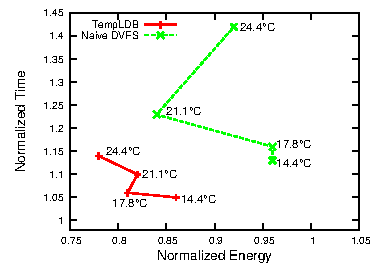
\includegraphics[width=0.3\textwidth]{../figures/ft_par.pdf}
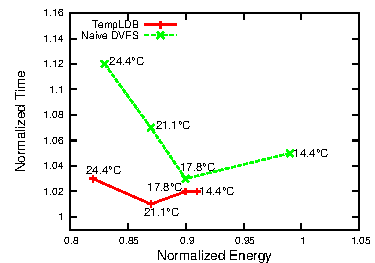
\includegraphics[width=0.3\textwidth]{../figures/jacobi_par.pdf}
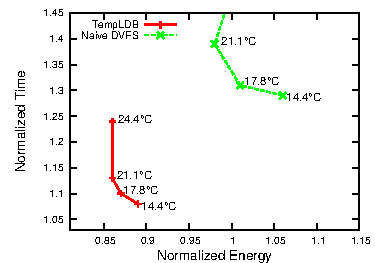
\includegraphics[width=0.3\textwidth]{../figures/wave_par_bk.pdf}
\pause
\begin{block}{Upcoming Technique}
Set power threshold on newer Intel CPUs, load balance as overloads appear
\end{block}
\end{frame}


